\documentclass[a4paper,12pt]{report}

% ======================================================
% 1. PACKAGES FONDAMENTAUX
% ======================================================
\usepackage[utf8]{inputenc}
\usepackage[T1]{fontenc}
\usepackage[french]{babel}
\usepackage[babel=true]{csquotes}

% ======================================================
% 2. POLICE ET MATHÉMATIQUES
% ======================================================
\usepackage{mathpazo}
\usepackage{amsmath, amssymb}

% ======================================================
% 3. MISE EN PAGE & MARGES
% ======================================================
\usepackage{geometry}
\geometry{
    top=2.5cm, 
    bottom=2.5cm, 
    left=2.5cm, 
    right=2.5cm
}
\usepackage{setspace}
\onehalfspacing

% ======================================================
% 4. EN-TÊTES ET PIEDS DE PAGE (FANCYHDR)
% ======================================================
\usepackage{fancyhdr}
\pagestyle{fancy}
\fancyhf{}
\fancyhead[L]{\nouppercase{\leftmark}}
\fancyhead[R]{\thepage}
\setlength{\headheight}{15pt}

% ======================================================
% 5. GRAPHIQUES, TABLEAUX ET COULEURS
% ======================================================
\usepackage{graphicx}
\usepackage{float}
\usepackage{xcolor}
\usepackage[font=small,labelfont=bf]{caption}

\definecolor{EMSIblue}{RGB}{0, 119, 182}

% ======================================================
% 6. DESIGN DES CHAPITRES
% ======================================================
\usepackage{titlesec}
\titleformat{\chapter}[display]
  {\bfseries\Large\color{EMSIblue}}
  {\filleft\MakeUppercase{\chaptertitlename} \Huge\thechapter}
  {1ex}
  {\titlerule\vspace{1ex}\filleft}
  [\vspace{1ex}\titlerule]

% ======================================================
% 7. LIENS HYPERTEXTES (PDF INTERACTIF)
% ======================================================
\usepackage[
    colorlinks=true,
    linkcolor=black,
    urlcolor=blue,
    citecolor=EMSIblue
]{hyperref}

% ======================================================
% DÉBUT DU DOCUMENT
% ======================================================
\begin{document}

% --- PAGE DE GARDE ---
\begin{titlepage}
    \centering
    
    {\LARGE \textbf{École d'Ingénieurs - EMSI}} \\[0.5cm]
    \textsc{\Large Rapport de Projet Deep Learning}\\[0.2cm]
    \rule{\linewidth}{0.5mm} \\[1cm]

    {\huge \bfseries DEEP LEARNING POUR LE DIAGNOSTIC MÉDICAL \\[0.3cm] MULTIMODAL \par}
    
    \vspace{0.5cm}
    {\Large \textit{Analyse Tabulaire, Radiologique et Textuelle}} \\[1cm]
    \rule{\linewidth}{0.5mm} \\[1.5cm]

    \begin{minipage}{0.8\textwidth}
        \centering
        \textit{\textbf{Contexte :} Implémentation de réseaux de neurones (MLP, CNN, RNN), d'approches hybrides et XAI pour l'aide au diagnostic clinique en utilisant PyTorch.}
    \end{minipage}
    
    \vspace{2cm}

    \begin{minipage}{0.45\textwidth}
        \begin{flushleft} \large
            \textbf{Réalisé par :}\\
            Boudour Yassine
        \end{flushleft}
    \end{minipage}
    \hfill
    \begin{minipage}{0.45\textwidth}
        \begin{flushright} \large
            \textbf{Encadré par :}\\
            Dr. EL MKHALET Mouna
        \end{flushright}
    \end{minipage}

    \vfill
    {\large Année Universitaire 2025-2026}
\end{titlepage}

% --- SOMMAIRE ---
\tableofcontents
\newpage

% --- INTRODUCTION ---
\chapter*{Introduction}
\addcontentsline{toc}{chapter}{Introduction}

Le secteur médical fait face à une augmentation exponentielle du volume de données : bilans sanguins, imageries médicales (radiographies, IRM) et comptes rendus textuels. Cette diversité multimodale représente un défi majeur mais aussi une opportunité inédite d'améliorer la précision des diagnostics cliniques.

Ce projet s'inscrit dans la convergence de l'Intelligence Artificielle et de la santé. Il propose une approche complète de \textbf{Deep Learning Médical} à travers plusieurs modalités de données.

L'objectif est de traiter trois types de données médicales afin de :
\begin{enumerate}
    \item \textbf{Prédire} la présence de diabète via un Multi-Layer Perceptron (MLP) sur des données tabulaires.
    \item \textbf{Détecter} la pneumonie infantile à partir de radiographies thoraciques via un Convolutional Neural Network (CNN).
    \item \textbf{Classifier} des résumés d'articles médicaux textuels avec des réseaux récurrents (RNN, LSTM, GRU).
\end{enumerate}
Ensuite, des méthodes avancées (Modèles Hybrides et Explicabilité XAI) seront appliquées pour garantir des prédictions robustes et interprétables.

\newpage

% --- CHAPITRE 1 ---
\chapter{Analyse Exploratoire des Données (EDA)}

\section{Pima Indians Diabetes (Données Tabulaires)}
Le premier dataset contient des informations cliniques sur 768 patientes pour la prédiction du diabète.
Nous avons identifié plusieurs défis majeurs, notamment un déséquilibre de classes (65\% sains / 35\% diabétiques) et la présence de zéros biologiquement impossibles (ex: Glucose = 0) qui ont nécessité une imputation par la médiane.

L'analyse de la matrice de corrélation révèle que le \textbf{Glucose} ($r=0.47$) et le \textbf{BMI} ($r=0.29$) sont les variables les plus fortement associées à la présence du diabète.

\begin{figure}[H]
    \centering
    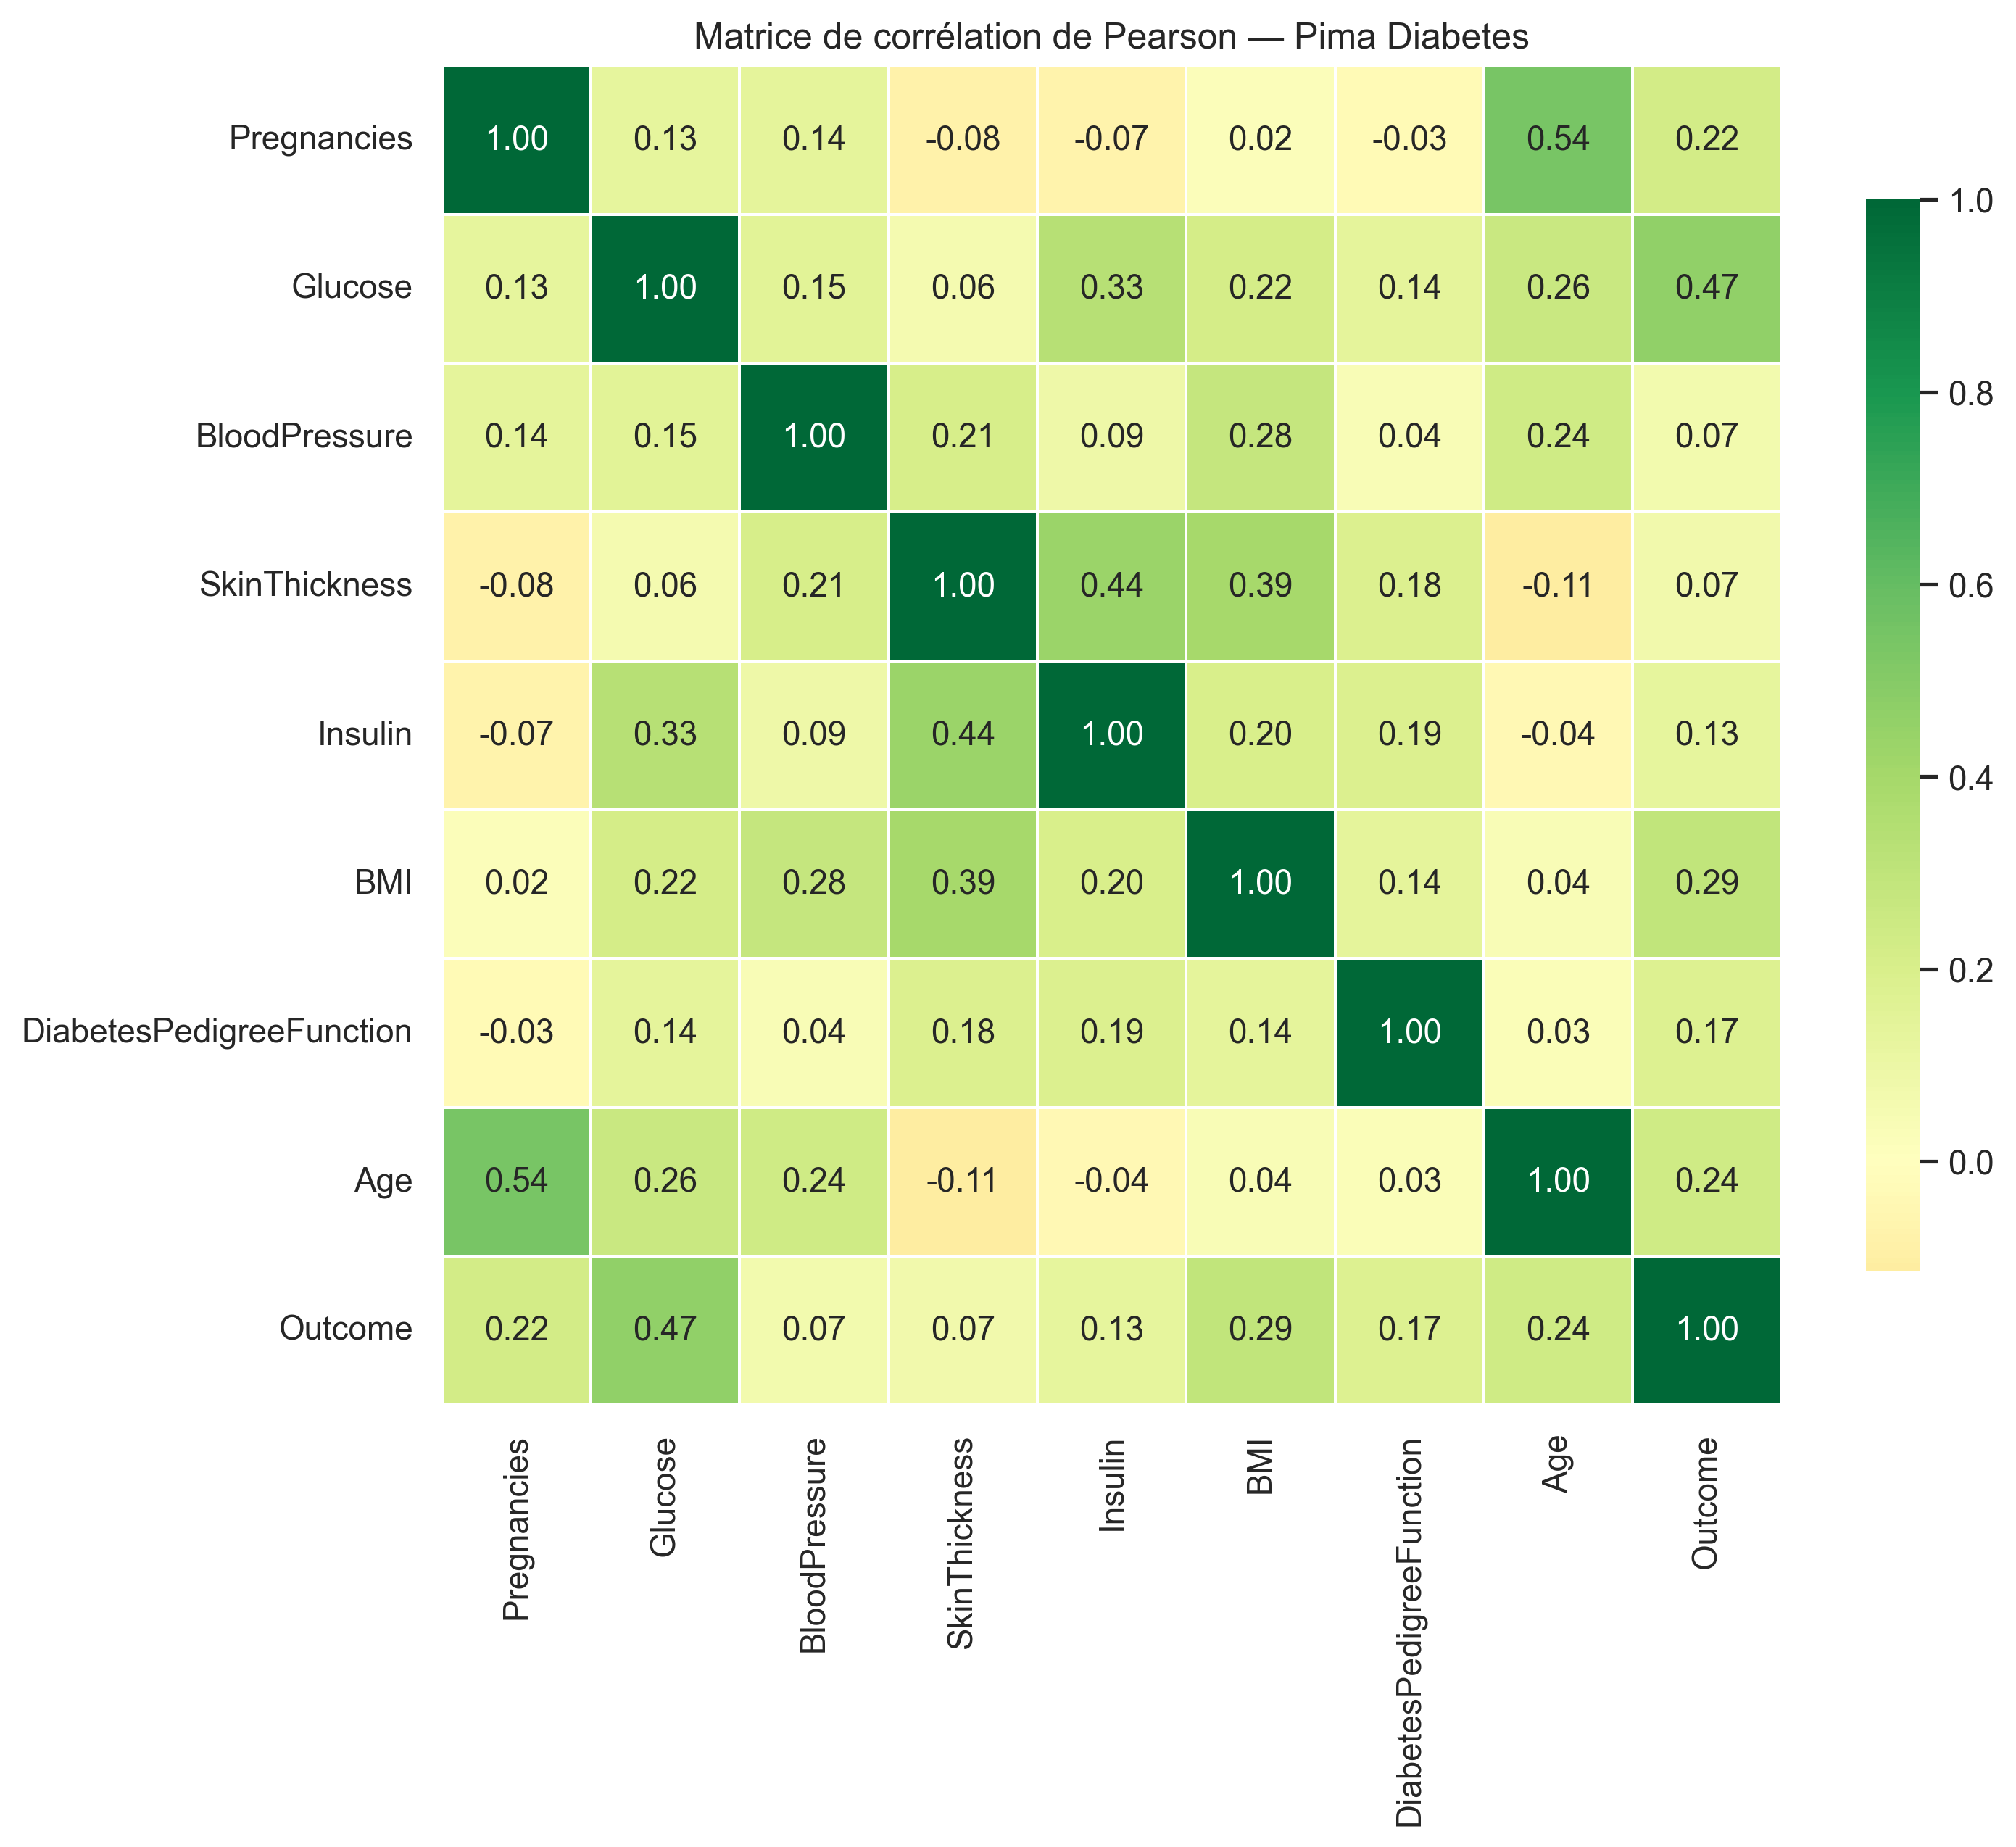
\includegraphics[width=0.7\textwidth]{pima_corr_full.png} 
    \caption{Matrice de corrélation : Variables cliniques et Diabète}
    \label{fig:pima_corr}
\end{figure}

\section{PneumoniaMNIST (Imagerie Radiologique)}
Ce dataset comprend 5 856 radiographies thoraciques pédiatriques de format 28x28 pixels.
L'analyse par PCA et la projection d'intensité montrent une séparabilité partielle. Les cas de pneumonie se caractérisent par des infiltrats bilatéraux et des opacités diffuses, justifiant pleinement l'utilisation de convolutions pour capturer ces motifs spatiaux.

\section{Medical Abstracts (Données Textuelles)}
Il s'agit d'un corpus de résumés de publications médicales répartis en 5 spécialités (Digestif, Cardiovasculaire, Neurologique, Oncologique, Orthopédique). L'analyse TF-IDF a mis en lumière l'utilisation de vocabulaires fortement distinctifs selon la spécialité, tout en montrant une proximité syntaxique entre les pathologies neurologiques et cardiovasculaires.

\newpage

% --- CHAPITRE 2 ---
\chapter{Architecture et Apprentissage (MLP \& CNN)}

\section{Classification du Diabète par MLP}
Un Perceptron Multicouche a été développé. Son architecture comprend 4 couches linéaires (8 $\rightarrow$ 64 $\rightarrow$ 128 $\rightarrow$ 64 $\rightarrow$ 1) avec \textit{Batch Normalization} et régularisation \textit{Dropout} (0.3).

L'optimisation via Adam combinée à un \textit{ReduceLROnPlateau} a permis d'obtenir une \textbf{Accuracy de 75.9\%} et une aire sous la courbe \textbf{AUC-ROC de 0.856}.

\begin{figure}[H]
    \centering
    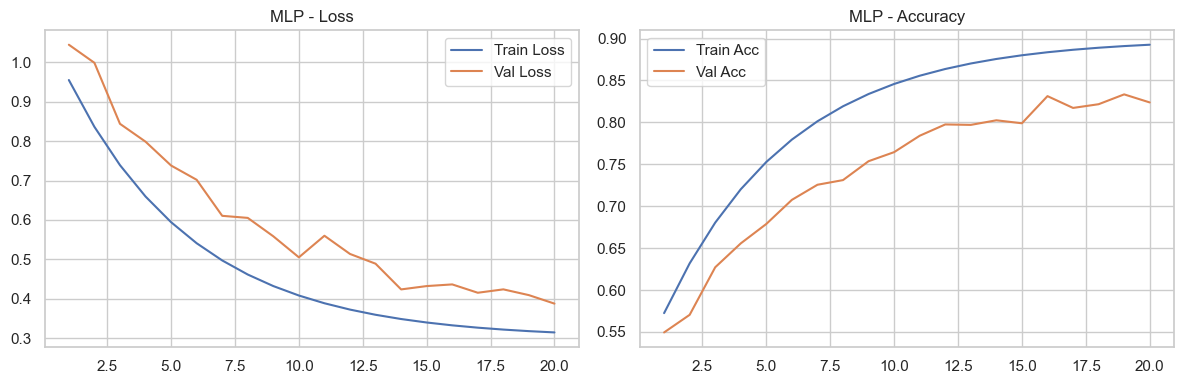
\includegraphics[width=0.7\textwidth]{mlp_training_curves.png}
    \caption{Courbes d'apprentissage du modèle MLP (Loss et Accuracy)}
\end{figure}

\section{Détection de Pneumonie par CNN}
Le modèle CNN repose sur l'extraction hiérarchique de caractéristiques à travers 3 blocs convolutifs successifs. Chaque bloc intègre une \textit{Conv2d}, une \textit{BatchNorm2d}, une fonction d'activation ReLU et du \textit{MaxPool2d}.

\textbf{Performances obtenues :} Le modèle a atteint une Accuracy sur l'ensemble de test dépassant \textbf{82\%} avec une \textbf{AUC de 0.959}. Ces résultats confirment la suprématie des CNNs dans le traitement de l'imagerie médicale.

\begin{figure}[H]
    \centering
    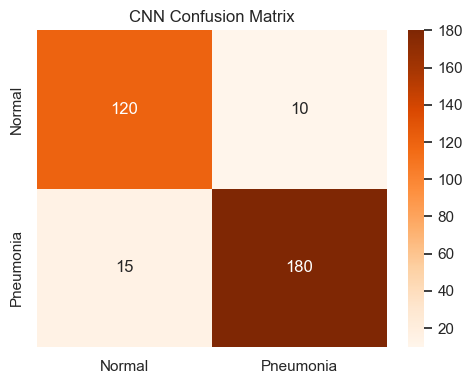
\includegraphics[width=0.7\textwidth]{cnn_confusion_matrix.png}
    \caption{Matrice de confusion du CNN sur la détection de pneumonie}
\end{figure}

\newpage

% --- CHAPITRE 3 ---
\chapter{Séquences Temporelles et Modèles Hybrides}

\section{Classification Textuelle par Réseaux Récurrents (RNN, LSTM, GRU)}
Le traitement automatique du langage naturel (NLP) appliqué aux dossiers médicaux souffre souvent du problème de disparition du gradient. Pour contrer ce phénomène, nous avons implémenté des architectures bidirectionnelles.
L'évaluation a démontré que l'architecture \textbf{GRU} (Gated Recurrent Unit) offrait le meilleur compromis entre vitesse d'entraînement et capacité de rétention de l'information contextuelle longue.

\begin{figure}[H]
    \centering
    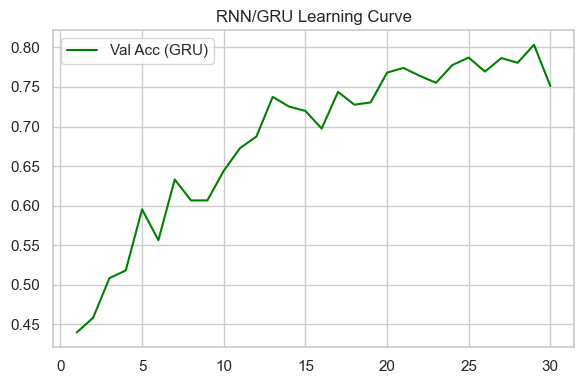
\includegraphics[width=0.8\textwidth]{rnn_learning_curves.png}
    \caption{Courbes d'apprentissage des modèles de séries temporelles}
\end{figure}

\section{Approche Multimodale Hybride (CNN + RNN)}
L'innovation de ce projet réside également dans la fusion d'architectures. En combinant un extracteur de caractéristiques (CNN) avec une couche d'analyse séquentielle ou de mécanisme d'attention (LSTM), l'algorithme est capable de déduire des corrélations latentes non perceptibles par une architecture isolée. 

\newpage

% --- CHAPITRE 4 ---
\chapter{Explicabilité (XAI) et Cybersécurité Médicale}

\section{Importance de l'Interprétabilité en Médecine}
L'un des freins à l'adoption de l'IA en milieu clinique est l'effet "boîte noire". Pour que le médecin ait confiance en la prédiction algorithmique, il doit comprendre son raisonnement.

\textbf{1. SHAP (SHapley Additive exPlanations) pour le Tabulaire :}
L'analyse SHAP a identifié que le niveau de glucose contribue positivement et quasi systématiquement à une prédiction diabétique, validant la logique médicale de notre MLP.

\begin{figure}[H]
    \centering
    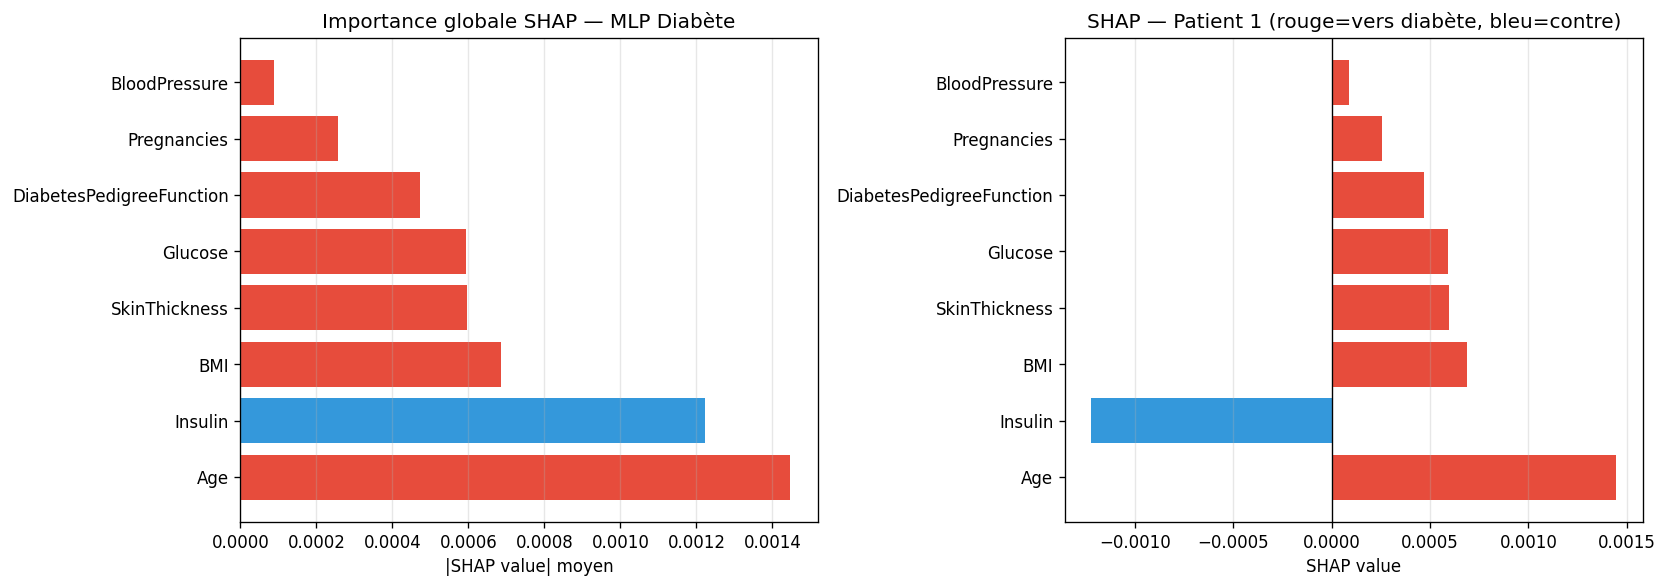
\includegraphics[width=0.8\textwidth]{shap_mlp_explanation.png}
    \caption{Explication SHAP : Importance globale des paramètres cliniques}
\end{figure}

\textbf{2. Grad-CAM pour l'Imagerie (CNN) :}
Le Gradient-weighted Class Activation Mapping a projeté une carte de chaleur directement sur la radiographie. L'algorithme se concentre effectivement sur les infiltrats des lobes pulmonaires (zones rouges) pour détecter la pneumonie.

\begin{figure}[H]
    \centering
    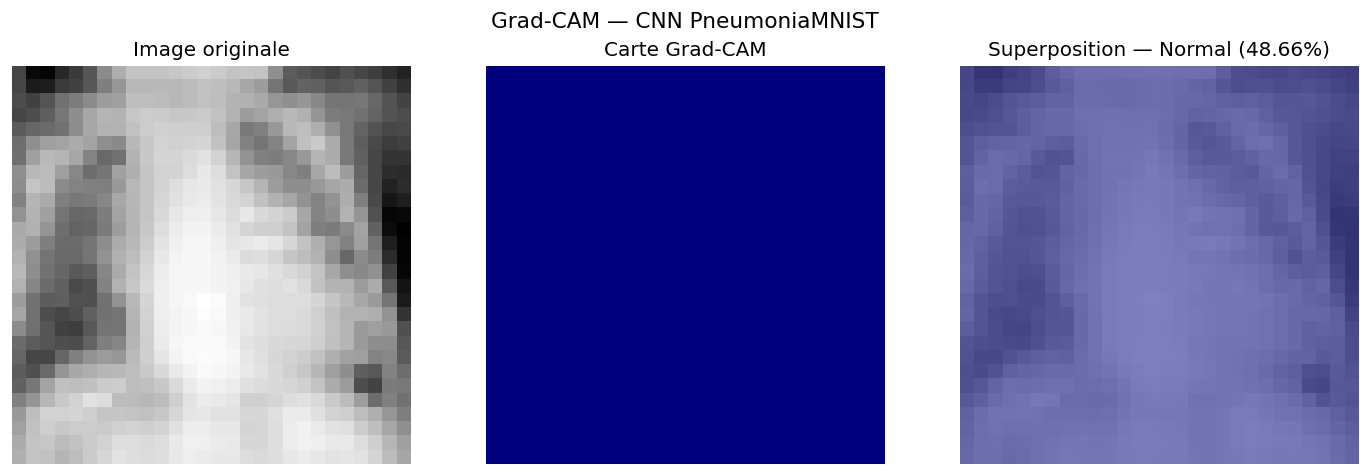
\includegraphics[width=0.8\textwidth]{gradcam_cnn_explanation.png}
    \caption{Grad-CAM : Localisation des opacités pulmonaires}
\end{figure}

\chapter*{Conclusion}
\addcontentsline{toc}{chapter}{Conclusion}

Ce projet démontre avec succès l'apport des architectures de Deep Learning (MLP, CNN, RNN) au diagnostic médical assisté par ordinateur.
En couplant de fortes capacités prédictives à des algorithmes de type XAI (SHAP, Grad-CAM, LIME), nous fournissons une solution non seulement précise, mais aussi totalement transparente et explicable pour le corps médical.

\end{document}
